\documentclass[12pt,addpoints]{exam}
\usepackage[utf8]{inputenc}
\usepackage{lastpage}
\usepackage{amsmath}
\usepackage{amsfonts}
\usepackage{amssymb}
\usepackage{enumerate}
\usepackage{mdframed}
\usepackage{array}
\usepackage{graphics}
\usepackage{graphicx}
\usepackage{listings}
\usepackage{tikz}
\usetikzlibrary{arrows}
\usepackage{algpseudocode}

% Paramètres globaux
\bonuspointpoints{point \emph{bonus}}{points \emph{boni}}
\parindent 0cm
\hqword{Question}
\hpword{Sur}
\hsword{Note}
\htword{Total}

% Réponses
%\printanswers

% En-tête et pieds de page
\headrule
\cfoot{\thepage /\pageref{LastPage}}
\lhead{CS Games --- Informatique théorique}
\rhead{Hiver 2016}
\newcommand{\headrulewidth}{0.4pt}
\newcommand{\footrulewidth}{0.4pt}

% Raccourcis
\newcommand{\bigo}{\mathcal{O}}
\newcommand{\N}{\mathbb{N}}
\newcommand{\R}{\mathbb{R}}

% Algorithmes
\algrenewcommand\algorithmicwhile{\textbf{tant que}}
\algrenewcommand\algorithmicfunction{\textbf{fonction}}
\algrenewcommand\algorithmicend{\textbf{fin}}
\algrenewcommand\algorithmicdo{\textbf{faire}}
\algrenewcommand\algorithmicfor{\textbf{pour}}
\algrenewcommand\algorithmicif{\textbf{si}}
\algrenewcommand\algorithmicelse{\textbf{sinon}}
\algrenewcommand\algorithmicthen{\textbf{alors}}
\algrenewcommand\algorithmicreturn{\textbf{retourner}}
\algrenewcommand\algorithmicrepeat{\textbf{faire}}
\algrenewcommand\algorithmicuntil{\textbf{tant que}}
\newcommand{\enteteproc}[2]{\vskip\baselineskip \hspace*{\fill} \algorithmicprocedure~\Call{#1}{#2} \hspace*{\fill} \vskip\baselineskip}
\newcommand{\entetefunc}[3]{\vskip\baselineskip \hspace*{\fill} \algorithmicfunction~\Call{#1}{#2} : #3 \hspace*{\fill} \vskip\baselineskip}

\begin{document}
	
\allowdisplaybreaks

\ifprintanswers
  \vskip 1.2cm
  \centerline{\large\underline{\textbf{Solution de l'épreuve}}}
  \vskip 0.5cm
\else
  \vskip 1.2cm
  \centerline{\large\underline{\textbf{Épreuve d'informatique théorique}}}
  \vskip 1.2cm
\fi

\ifprintanswers
\else
  \begin{center} \gradetable[h] \end{center}
\fi

\begin{questions}

% Graphes
\uplevel{Les questions suivantes portent sur la théorie des graphes.
Un \emph{graphe simple} est un couple $G = (V,E)$ où $V$ est son ensemble de \emph{sommets} et $E \subseteq \mathcal{P}_2(V)$ est son ensemble d'\emph{arêtes}, où $\mathcal{P}_2(V)$ dénote l'ensemble des paires d'éléments distincts de $V$. Par exemple, le graphe $G = (V,E)$ défini par les ensembles
$$V = \{a,b,c,d\} \quad \text{et} \quad E = \{\{a,b\}, \{a,c\}, \{b,c\}, \{c,d\}\}$$
est représenté à la figure \ref{F:graphe}. À noter que dans un graphe simple, il n'y a pas d'arête multiple ni de boucle (une arête d'un sommet vers lui-même).}

% Familles de graphes
\question
Certaines familles de graphes simples sont souvent utilisées. En voici quelques-unes (voir figure~\ref{F:familles})~:
\begin{enumerate}[(i)]
  \item Pour tout entier $n \geq 1$, le graphe \emph{complet} de $n$ sommets $K_n$;
  \item Pour tout entier $n \geq 3$, le \emph{cycle} de $n$ sommets $C_n$;
  \item Pour tout entier $n \geq 3$, la \emph{roue} de $n + 1$ sommets $W_n$;
  \item Pour tout entier $n \geq 1$, l'\emph{hypercube} de dimension $n$ est noté $H_n$;
  \item Pour toute paire d'entiers $m,n \geq 1$, le graphe \emph{biparti complet} $K_{m,n}$;
\end{enumerate}
Pour toutes valeurs $n$ et $m$ bien définies, donnez le nombre d'arêtes des graphes suivants~:
\begin{parts}
  \part $K_n$;
  \part $C_n$;
  \part $W_n$;
  \part $h_n$;
  \part $K_{m,n}$.
\end{parts}

% Transversaux d'arêtes
\question
Soit $G = (V,E)$ un graphe simple. On dit d'un ensemble de sommets $U \subseteq V$ qu'il est un \emph{transversal d'arêtes} si chaque arête de $G$ a au moins une de ses extrémités dans $U$, c'est-à-dire que pour toute arête $\{u,v\} \in E$, on a $u \in U$ ou $v \in U$. Par exemple, dans le graphe de la figure \ref{F:graphe}, l'ensemble $\{a,c\}$ est un transversal d'arêtes. Un transversal d'arête $U$ est dit \emph{minimum} pour $G$ s'il n'existe aucun transversal d'arêtes $U'$ de plus petite cardinalité, c'est-à-dire tel que $|U'| < |U|$.

Pour toutes valeurs de $n$ et $m$ bien définies, donnez la taille d'un transversal d'arêtes minimum des graphes suivants~:
\begin{parts}
  \part $K_n$;
  \part $C_n$;
  \part $W_n$;
  \part $h_n$;
  \part $K_{m,n}$.
\end{parts}

% Problème HAMD
\question
On dit d'un graphe $G$ qu'il est \emph{hamiltonien} s'il admet au moins un cycle passant par chaque sommet \textbf{exactement} une fois.

Soit HAMD le problème de \emph{décider} si un graphe simple $G$ est hamiltonien ou non et soit HAM le problème de \emph{trouver} un cycle hamiltonien dans un graphe $G$ (on retourne la valeur \emph{rien} si un tel cycle n'existe pas). Autrement dit, on considère les deux fonctions suivantes~:
\begin{itemize}
  \item \Call{EstHamiltonien}{$G$ : graphe} : booléen;
  \item \Call{CycleHamiltonien}{$G$ : graphe} : cycle ou \emph{rien}.
\end{itemize}
Montrez que les deux problèmes sont de même difficulté à complexité polynomiale près. En d'autres termes, si $\textsc{EstHamiltonien}$ utilise un temps constant, alors on peut implémenter $\textsc{CycleHamiltonien}$ de telle sorte qu'elle utilise un temps polynomial (et vice-versa).
\begin{solution}
Supposons d'abord que \textsc{CycleHamiltonien} utilise un temps constant. Alors la fonction
\begin{algorithmic}[1]
  \Function{EstHamiltonien}{$G$ : graphe} : booléen
    \State \Return \Call{CycleHamiltonien}{$G$}~$\neq$~rien
  \EndFunction
\end{algorithmic}
a également une complexité constante.

Réciproquement, supposons que \textsc{EstHamiltonien} utilise un temps constant et considérons la fonction suivante~:
\begin{algorithmic}[1]
  \Function{CycleHamiltonien}{$G = (V,E)$ : graphe} : cycle ou rien
    \If{$\neg \Call{EstHamiltonien}{G}$}
      \State \Return rien
    \Else
      \While{il existe $v \in V$ tel que $\deg(v) > 2$}
        \State Soit $v$ un sommet de degré au moins $3$
        \For{$u \in G.\Call{Voisins}{v}$}
          \State Soit $H$ le graphe obtenu de $G$ en supprimant $\{u,v\}$
          \If{$\Call{EstHamiltonien}{H}$}
            \State $G \leftarrow H$
          \EndIf
        \EndFor
      \EndWhile
      \State \Return l'unique cycle de $G$
    \EndIf
  \EndFunction
\end{algorithmic}
Sa complexité est de $\bigo(m(m + n)) = \bigo(m^2)$ qui est bien polynomiale.
\end{solution}
\end{questions}

\begin{figure}
  \centering
  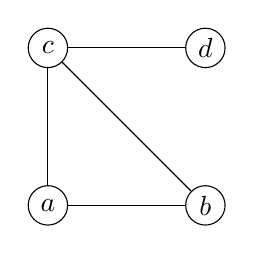
\begin{tikzpicture}[sommet/.style={draw, circle, inner sep=0pt, minimum size=5mm}]
    % Sommets
    \node[sommet] at (0,0) (a) {$a$};
    \node[sommet] at (2,0) (b) {$b$};
    \node[sommet] at (0,2) (c) {$c$};
    \node[sommet] at (2,2) (d) {$d$};
    % Arêtes
    \path (a) edge (b) edge (c);
    \path (c) edge (b) edge (d);
  \end{tikzpicture}
  \caption{Le graphe $G = (V,E)$, où $V = \{a,b,c,d\}$ et $E = \{\{a,b\}, \{a,c\}, \{b,c\}, \{c,d\}\}$.}\label{F:graphe}
\end{figure}

\end{document}
